
\documentclass[preprint,12pt]{elsarticle}

\usepackage[spanish]{babel}
\usepackage{amssymb}
\usepackage{graphicx}
\usepackage{lineno}
\usepackage[utf8]{inputenc}
\usepackage{url}
\usepackage{natbib}

\begin{document}
	
	\begin{frontmatter}

		\title{\huge  PROYECTO DE  ANALISIS Y  MEJORAMIENTO DE  SOFTWARE }
		\author{Katerin Merino Quispe              (2018060918)}
		\author{Percy Taquila                ()}
		\author{Abraham                ()}
		\author{Edwart                ()}
		\author{Liz                ()}
		\address{Tacna, Perú}
		


%%INICIO abstract
\begin{abstract}
This document is intended to present patient care in a concise and clear way, diagnosing their possible disease with terms of software that would be carried out in the system. In this documentation, the requirements that will serve as a guide to develop the software in its different stages will be reflected, helping us to validate and inspect its construction, applying the Software quality.
Therefore, we will work with Sonarqube for the analysis of static code to analyze the code and find code errors, and security vulnerabilities. SonarSource's C char analysis has extensive coverage of well-established quality standards.  
\end{abstract}
%%FIN abstract


\end{frontmatter}
%%INICIO Introducción
\section{Antecedentes o Introducción}

El "Sistema de Diagnostico Medico" esta desarrollado para que la atención a los pacientes sean mas rápidas, ya que en esta pandemia hace que la atencion sea insufiente, falta de tiempo y con este sistema se busca atender mas rápido y de forma ordenada a los pacientes que vienen a sus consultas, con este sistema se diagnostica al paciente con los síntomas que nos diga en el momento de la consulta y dar como resultado su posible enfermedad que tiene y las recomendaciones que debe seguir para recuperarse.
%%FIN Introducción

%%INICIO Titulo
\section{Titulo}
"Sistema de Diagnostico Medico"
Propuesta de un sistema de atención al paciente diagnosticando su posible enfermedad.
%%FIN Titulo
%%INICIO Autores
\section{Autores}
\begin{itemize}
    \item Katerin Merino Quispe
    
\end{itemize}
%%FIN Autores
%%INICIO Planteamiento del problema
\section{Planteamiento del problema}
no se si ira un texto aqui

%%----------------------------------------------------------------------------------------------------------------------------------------------------------
	\subsection{\textbf{Problema}}
 La falta e insuficiencia de herramientas para el apoyo en el diagnóstico de enfermedades, además por la pandemia que está pasando el mundo entero la demanda de pacientes no está siendo cubierta. Es por ello que muchos pacientes no son atendidos, es por eso que se necesita un sistema para poder agilizar la atención hacia los pacientes en su caso sea.
%%-----------------------------------------------------------------------------
	\subsection{\textbf{Justificación }}
Crear un sistema de diagnóstico para las enfermedades es necesario debido a que puede ayudar al especialista a brindar una respuesta más rápida, la implementación de este sistema va a mejorar la gestión de los servicios y la atención.

%%-----------------------------------------------------------------------------
	\subsection{\textbf{ Alcance }}
El software a desarrollar describimos cada funcionalidad del proyecto que está orientado a las consultas que se realizaran las personas con síntomas de alguna enfermedad.

\section{Objetivos}
		\subsection{\textbf{ General }}
	 \begin{itemize}
		\item Desarrollar un sistema de diagnóstico médico para optimizar el tiempo  de respuesta del diagnóstico médico.
	 \end{itemize}
		\subsection{\textbf{Específicos }}
\begin{itemize}
	\item Que el diagnóstico médico muestre las posibles enfermedades de un paciente.
	\item Detectar que tipo de posible enfermedad tiene el paciente. 
	\item Almacenar el historial del paciente en la base de datos. 
	\end{itemize}

	\section{Referentes teóricos}
\begin{itemize} 
 \item (EN ESTA PARTE HAY QUE VER QUE PONER, COLOCAN PORFAVOR, LO DE ABAJO ES UNA GUIA)

    \item Hemos realizado una investigación en empresas relacionadas con el rubro de la ferretería, en este caso elegimos el caso de la empresa HELEO situada en el parque industrial de Tacna, donde pudimos observar como trabaja su sistema de COMPRA Y VENTA de productos.
	\begin{center}
	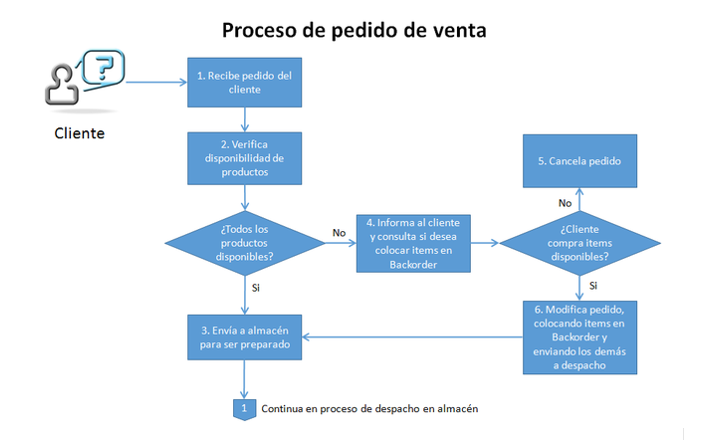
\includegraphics[width=12cm]{./imagen/1} 
	\end{center}
	\item Posee un anexo en la web de CATALOGO EN LINEA donde da una mayor promoción a sus productos antes de acudir a la tienda a comprarlos.
	\begin{center}
	
\includegraphics[width=12cm]{./imagen/2} 
	\end{center}
	\item Asimismo pudimos ver un detalle interesante que era un modulo de CONSULTA DE FACTURAS ELECTRONICAS VIA INTERNET para los clientes
	\begin{center}
	
\includegraphics[width=12cm]{./imagen/3} 
	\end{center}
\end{itemize}

\section{Desarrollo de la propuesta}
La calidad de código suele decirse que es un atributo interno de calidad, dado que no se hace visible al usuario. Pero llega un momento en el cual este atributo de calidad pasa de ser interno a externo, y esto se da cuando el hecho de tener modificar el código para hacer un cambio lleva mucho más tiempo del que debería. Con el fin de verificar la calidad interna de un sistema se suelen hacer análisis de código con SonarQube o herramientas similares. En este documento se muestra parte de de nuestro proyecto , donde básicamente  cuenta cómo hacer una prueba de concepto rápidamente usando una imagen Docker de SonarQube, y ejecutando el análisis desde SonarQube Scanner.
SonarQube, como tantas otras herramientas similares, permite realizar análisis estático de código fuente de manera automática, buscando patrones con errores, malas prácticas o incidentes. Además, realiza un cálculo de la deuda técnica. Dentro de las verificaciones que hacen herramientas como SonarQube, se encuentran las siguientes:
\begin{itemize}
	\item Detección de código duplicado..
	\item Falta de pruebas unitarias, falta de comentarios. 
	\item Código spaghetti, complejidad ciclomática, alto acoplamiento.
	\item Tamaño de archivos de código.
	\item Tamaño de métodos.
	\item No adecuación a estándares y convenciones de código.
	\item Vulnerabilidades conocidas de seguridad.
	
	Una muestra en Nuestro proyecto:
		
        \begin{center}
	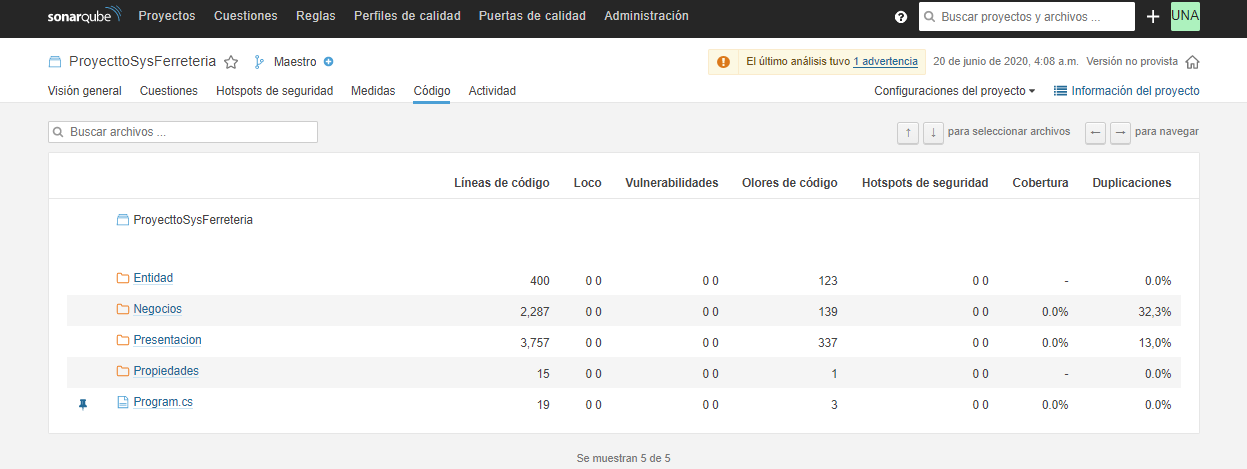
\includegraphics[width=12cm]{./imagen/7} 
	\end{center}
\end{itemize}

\subsection{\textbf{Tecnología de información  }}
		\begin{itemize}
	\item 	SQL SERVER: Microsoft SQL Server es un sistema de gestión de base de datos relacional, desarrollado por la empresa Microsoft. El lenguaje de desarrollo utilizado es Transact-SQL, una implementación del estándar ANSI del lenguaje SQL, utilizado para manipular y recuperar datos, crear tablas y definir relaciones entre ellas..
	\item 	C char : lenguaje de programación multiparadigma desarrollado y estandarizado por Microsoft. Es un lenguaje de programación creado para diseñar aplicaciones en la plataforma.NET.
	\item 	Visual Studio: es un entorno de desarrollo en diferentes sistemas operativos y compatibles con múltiples lenguajes de programación al igual que entornos de desarrollo web. 
	\end{itemize}
\subsection{\textbf{ Metodología, técnicas usadas  }}
UML es un lenguaje para hacer modelos y es independiente de los métodos de análisis y diseño. Existen diferencias importantes entre un método y un lenguaje de modelado. Un método es una manera explícita de estructurar el pensamiento y las acciones de cada individuo. Además, el método le dice al usuario qué hacer, cómo hacerlo, cuándo hacerlo y por qué hacerlo; mientras que el lenguaje de modelado carece de estas instrucciones. Los métodos contienen modelos y esos modelos son utilizados para describir algo y comunicar los resultados del uso del método.
          \begin{center}
	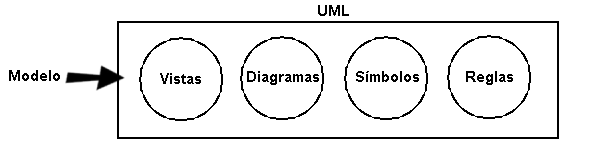
\includegraphics[width=12cm]{./imagen/5} 
	\end{center}
		
\section{Cronograma }

	\begin{center}
	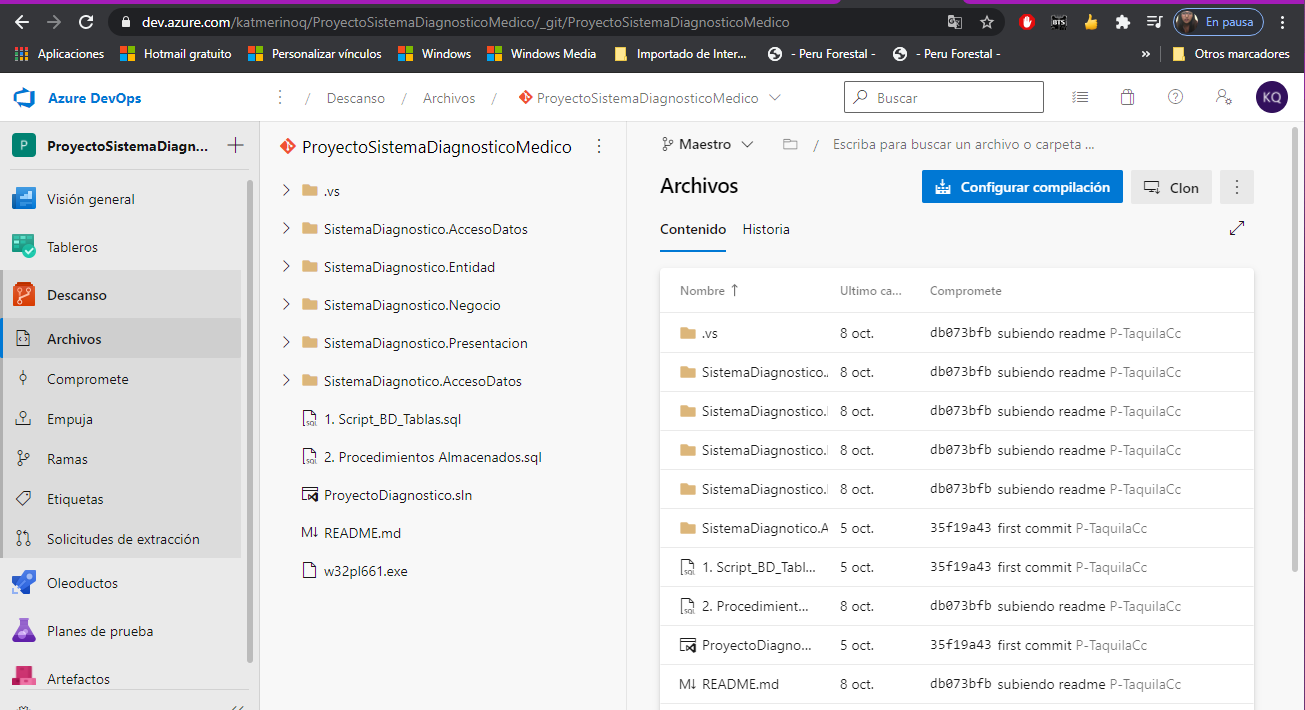
\includegraphics[width=12cm]{./imagen/20} 
	\end{center}

\section{Resultado Sonarqube}
	Definición de métricas
	\begin{itemize}
	    \item Código duplicado
	\begin{center}
	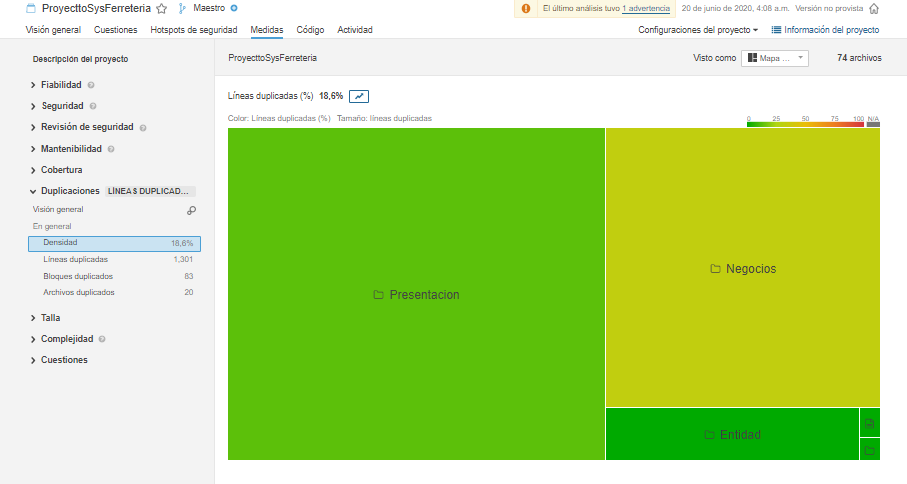
\includegraphics[width=12cm]{./imagen/8} 
	\end{center}
	\item Mantenibilidad
	\begin{center}
	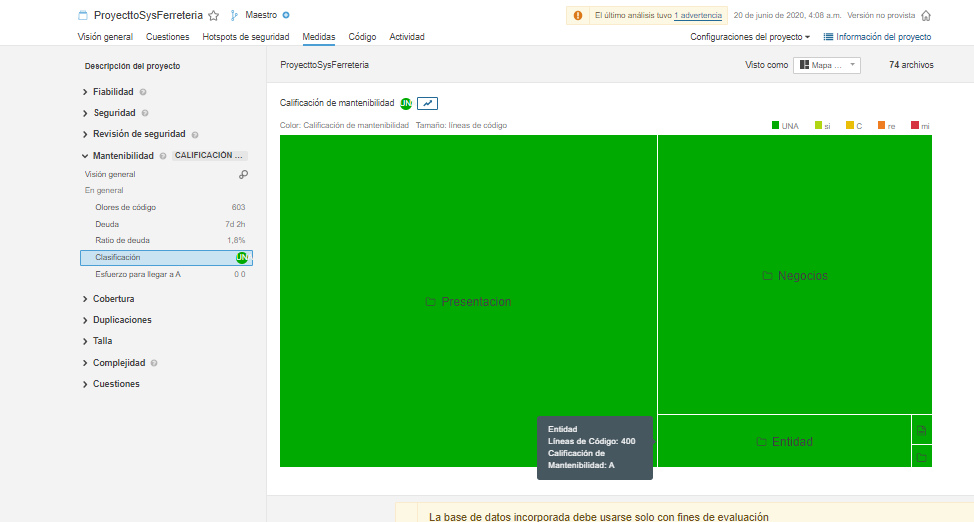
\includegraphics[width=12cm]{./imagen/9} 
	\end{center}
	\item Medida
		\begin{center}
	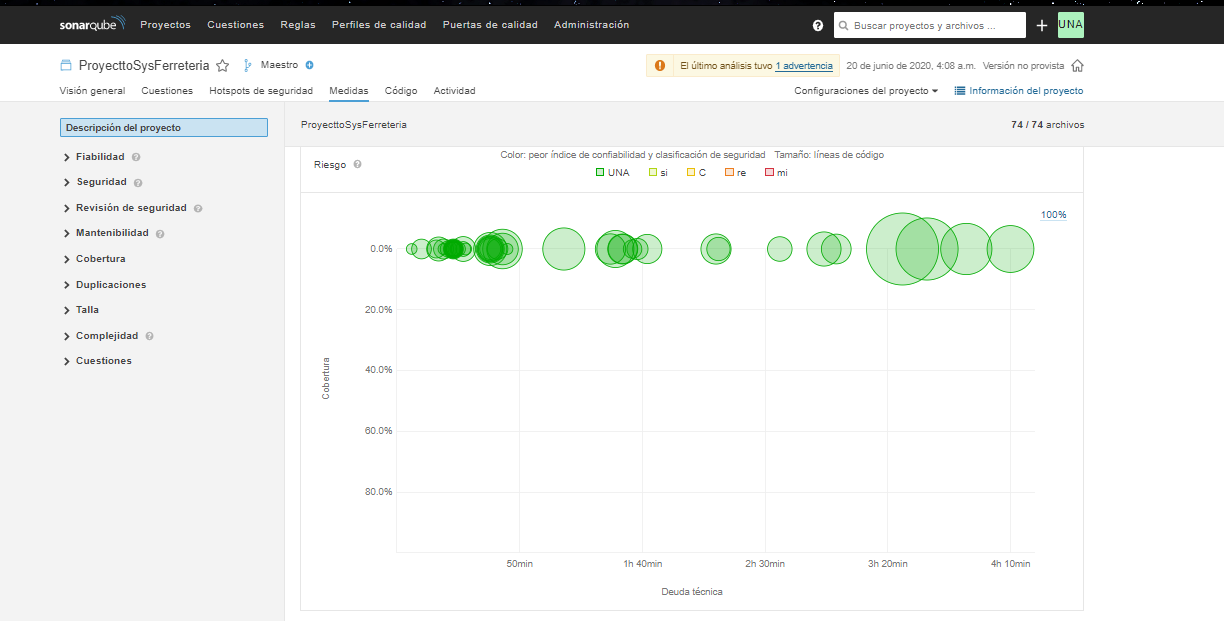
\includegraphics[width=12cm]{./imagen/10} 
	\end{center}
	\end{itemize}
\section{Desarrollo de Solución de Mejora}
\subsection{\textbf{ Casos de Uso de la aplicación}}
\begin{center}
	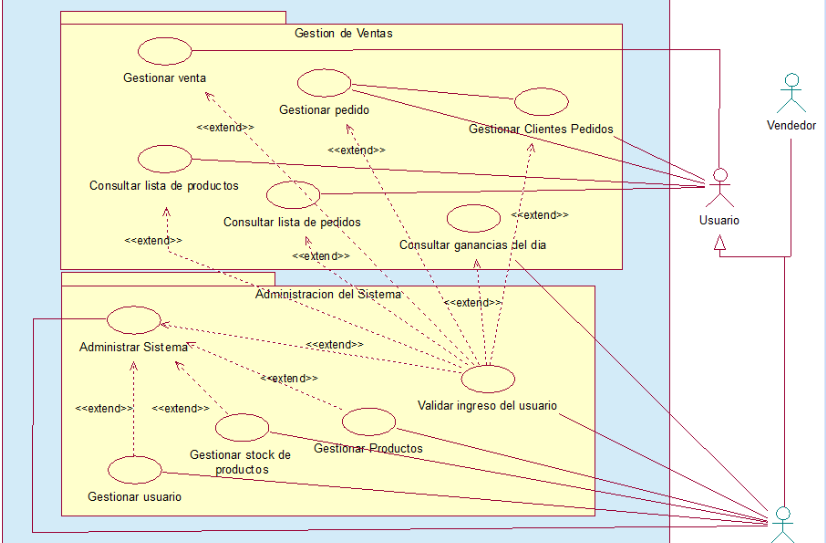
\includegraphics[width=12cm]{./imagen/casouso} 
	\end{center}
\subsection{\textbf{ Diagrama de Arquitectura de la aplicación }}



\begin{itemize}
\item Existen diferentes tipos de arquitectura o patrones a seguir para desarrollar un software, en este caso voy a explicar en que consiste la aqruitectura de 3 Capas , que ami parecer es la mas general o la mas basica para desarrollar.
	\item La Capa de Presentación : Donde se encuentran los formularios y la parte visual de la aplicación.
	\item 	La Capa de Negocios  : Donde se encuentra toda la logica del negocio y clases que las componete es decir, Entidades y controladoras)

	\item 	La Capa de Acceso a Datos: Donde se encuentra las conexiones y las transacciones que se utilizan para comunicarse con la base de datos.
	\end{itemize}
	\begin{center}
	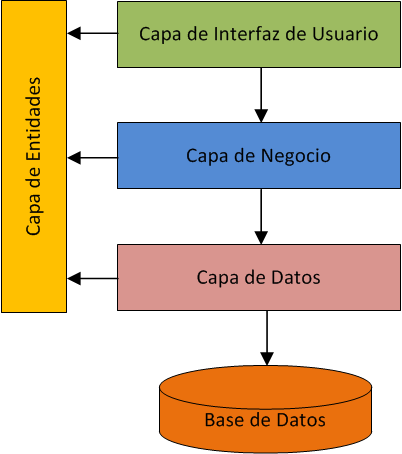
\includegraphics[width=7cm]{./imagen/23} 
	\end{center}
	\begin{center}
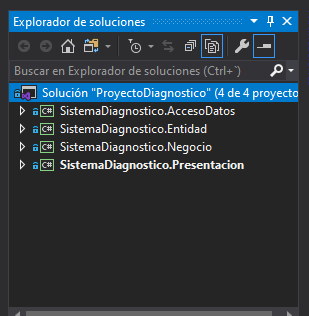
\includegraphics[width=7cm]{./imagen/4capas} 
	\end{center}
\subsection{\textbf{ Diagrama de Clases de la aplicación }}
\begin{center}
	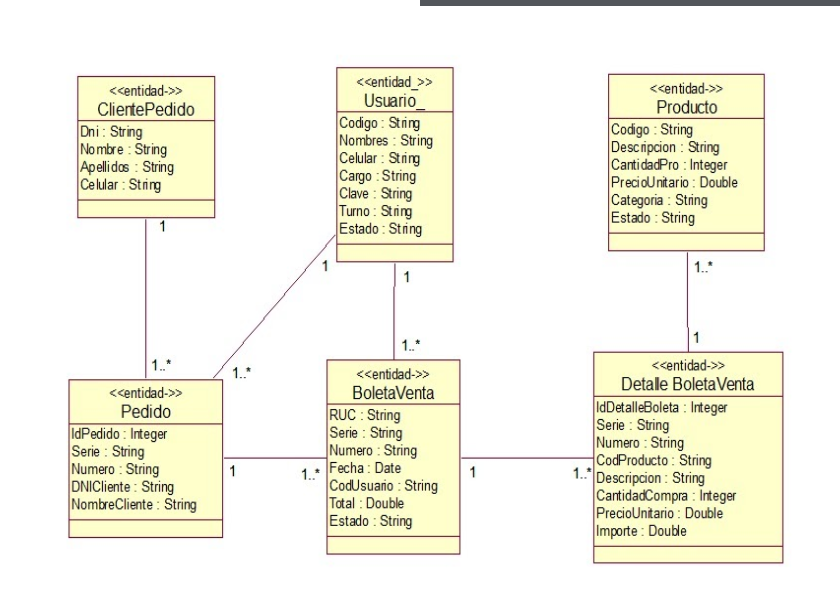
\includegraphics[width=12cm]{./imagen/diagrmclasesvistaprocesos} 
	
	\end{center}

\subsection{\textbf{  Metodos de pruebas implementados para coberturar la aplicación }}
\renewcommand{\labelenumi}{{\theenumi})}
\begin{enumerate}
\item  Pruebas Unitarias  
\begin{center}
	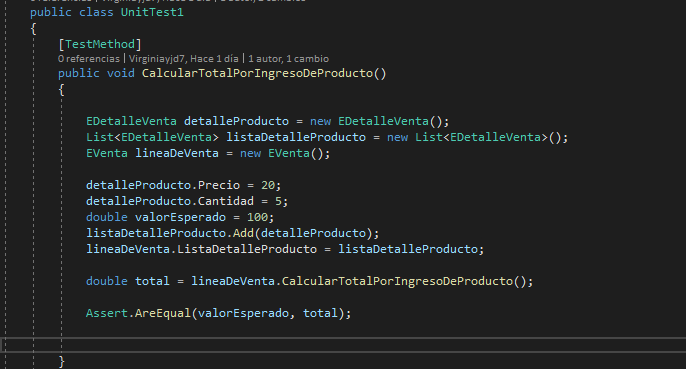
\includegraphics[width=12cm]{./imagen/calcular} 
	\end{center}
\begin{center}
	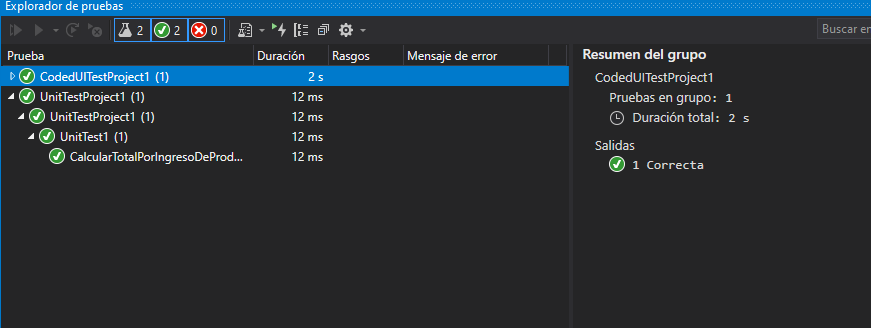
\includegraphics[width=12cm]{./imagen/pruebas} 
	\end{center}
\item  Pruebas de Interfaz 
\begin{center}
	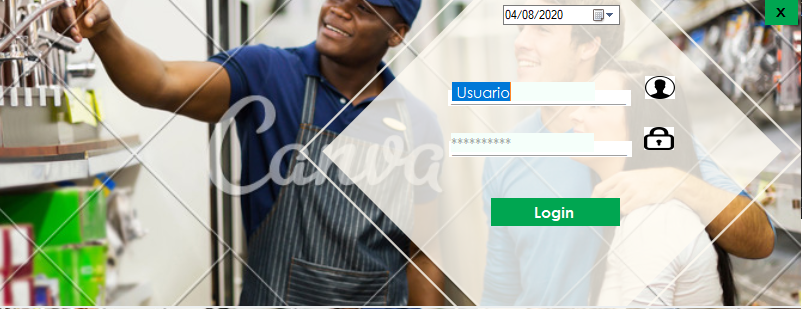
\includegraphics[width=12cm]{./imagen/interface} 
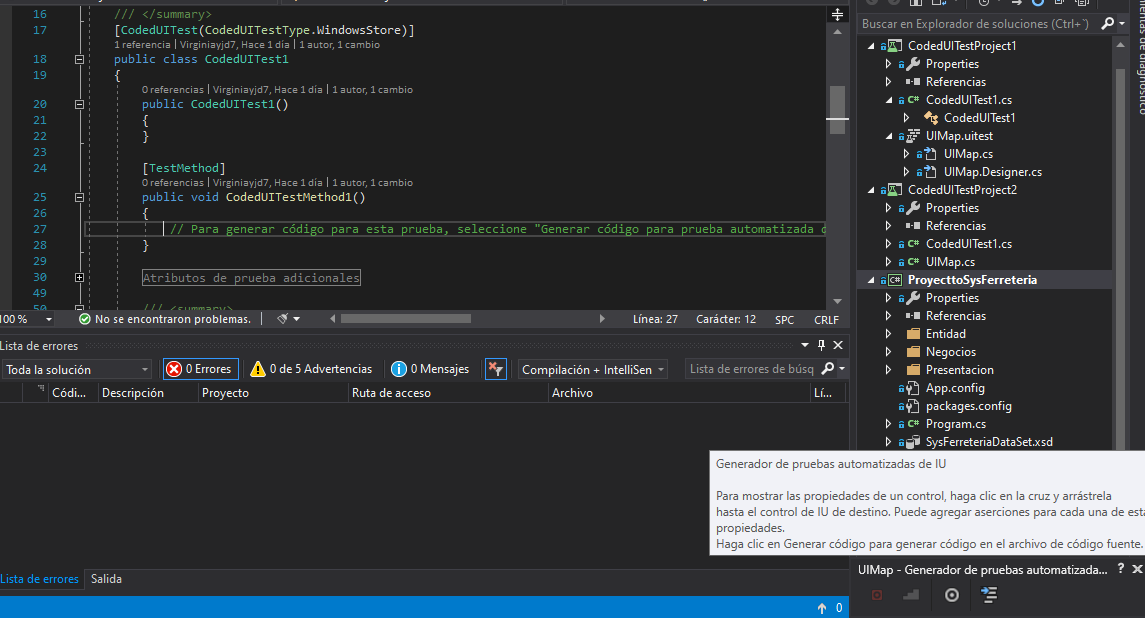
\includegraphics[width=12cm]{./imagen/f} 
	\end{center}
\item Pruebas basadas en Desarrollo Guiado por el Comportamiento
\end{enumerate}
\section{Desplegar las pruebas automatizas  Azure Devops y Git gub actions }
Para hacer la prueba se clonado desde el repositorio de GitHub el proyecto
\begin{itemize} 
    \item Para hacer la prueba se clonado desde el repositorio de GitHub el proyecto
	\begin{center}
	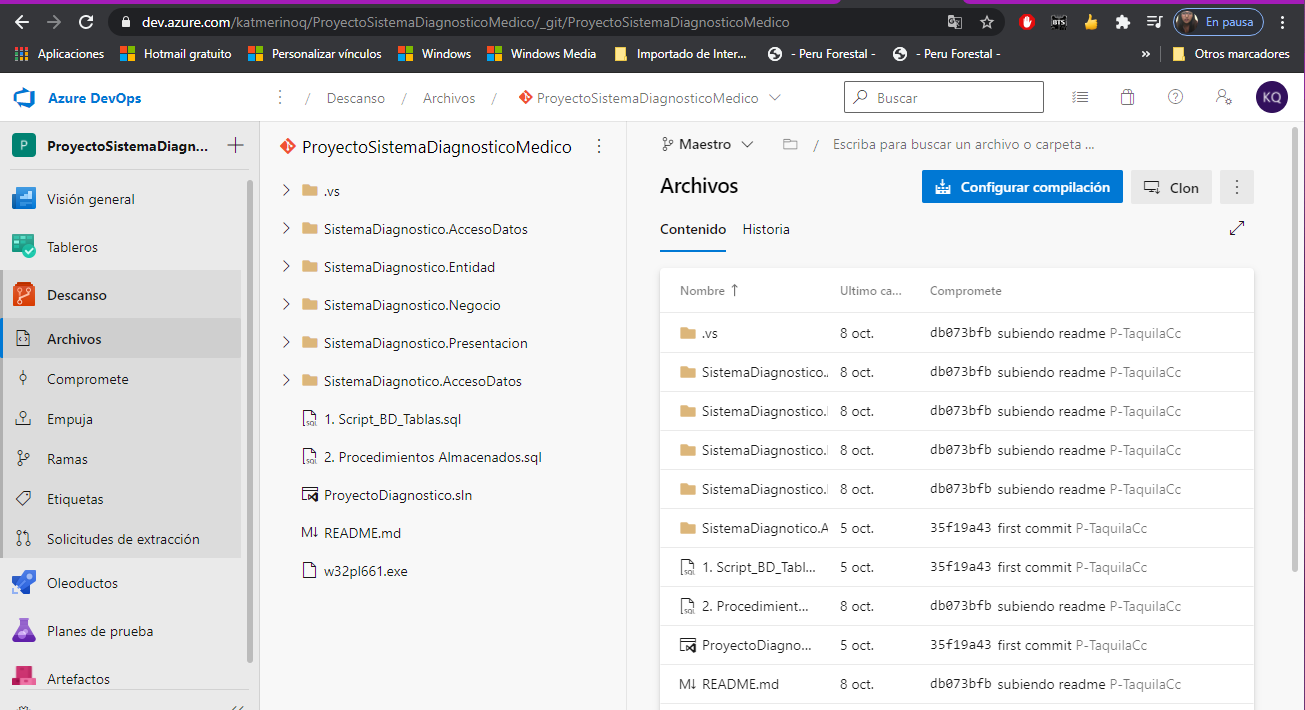
\includegraphics[width=12cm]{./imagen/20} 
	\end{center}
	\item se crea Pipelines
	\begin{center}
	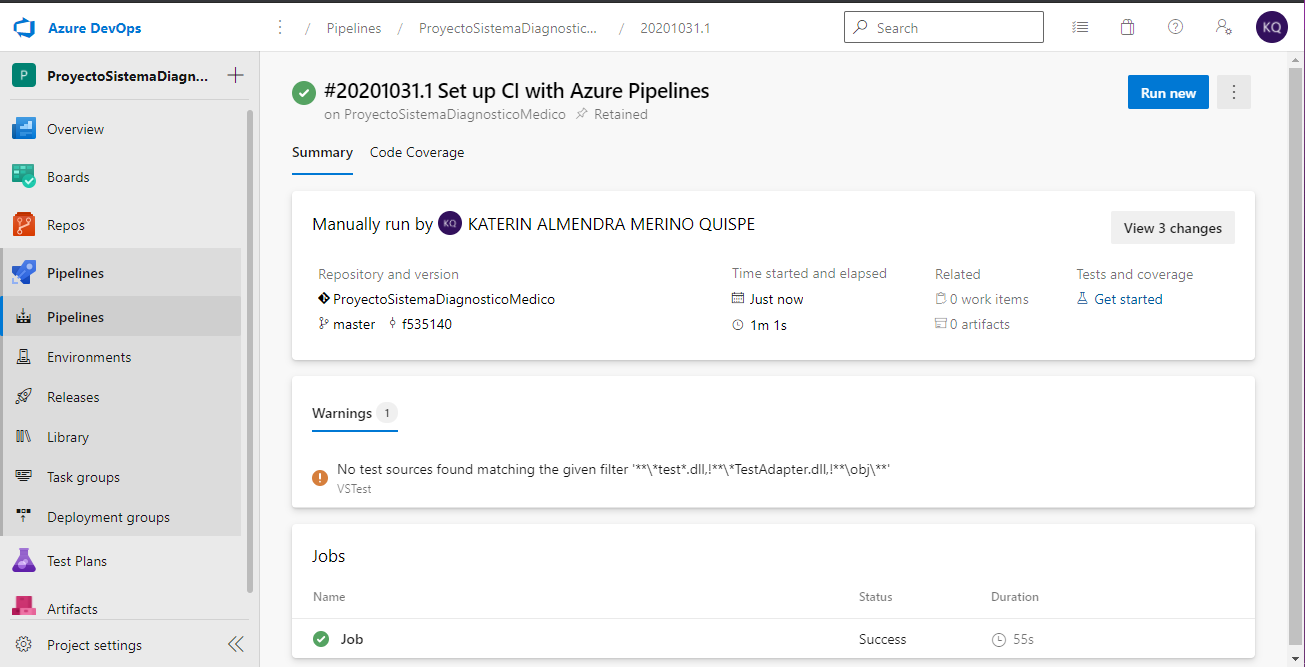
\includegraphics[width=12cm]{./imagen/21} 
	\end{center}
	\item y posteriorme a la ejecusion
	\begin{center}
	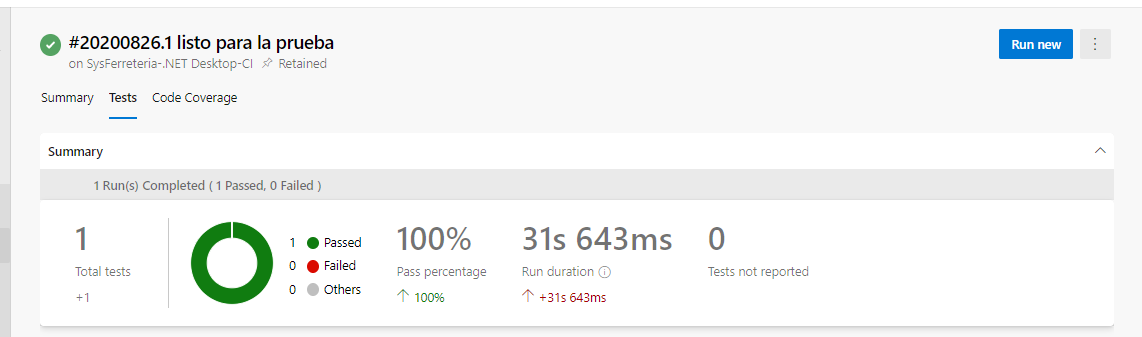
\includegraphics[width=12cm]{./imagen/22} 
	\end{center}
\end{itemize}
	\newpage
	
	\bibliography{BIBLIOGRAFIA}	

\end{document}

